\documentclass[fleqn,reqno,10pt]{article}


\usepackage[style=authoryear-comp, 
            natbib=true,     
            hyperref=true,    
            maxnames=3,       
            doi=false,        
            url=false,        
            sortcites=false,  
            ]{biblatex}
\bibliography{references}
\usepackage{subcaption}
\usepackage{booktabs}
\usepackage{xspace}
\usepackage[utf8]{inputenc}
\usepackage[sc,osf]{mathpazo}
\linespread{1.12}
\usepackage[width=16cm]{geometry}

% these packages are needed to insert results 
% obtained from R into the LaTeX document
\usepackage{pgfplotstable}
\usepackage{csvsimple}
\usepackage{siunitx}

% set the name of the folder in which the CSV files with 
% information from R is stored
\newcommand{\datafoldername}{R_data_4_TeX}

% the following code defines the convenience functions
% as described in the main text below

% rlgetvalue returns whatever is the in cell of the CSV file
% be it string or number; it does not format anything
\newcommand{\rlgetvalue}[4]{
  \csvreader[filter strcmp={\mykey}{#3},
             late after line = {{,}\ }, late after last line = {{}}]
            {\datafoldername/#1}{#2=\mykey,#4=\myvalue}{\myvalue}}

% rlgetvariable is a shortcut for a specific CSV file (myvars.csv) in which
% individual variables that do not belong to a larger chunk can be stored
\newcommand{\rlgetvariable}[1]{
  \csvreader[]{\datafoldername/myvars.csv}{#1=\myvar}{\myvar}\xspace
}

% rlnum format a decimal number
\newcommand{\rlnum}[2]{\num[output-decimal-marker={.},
                             exponent-product = \cdot,
                             round-mode=places,
                             round-precision=#2,
                             group-digits=false]{#1}}

\newcommand{\rlnumsci}[2]{\num[output-decimal-marker={.},
                          scientific-notation = true,
                             exponent-product = \cdot,
                             round-mode=places,
                             round-precision=#2,
                             group-digits=false]{#1}}

\newcommand{\rlgetnum}[5]{
  \csvreader[filter strcmp={\mykey}{#3},
             late after line = {{,}\ }, late after last line = {{}}]
            {\datafoldername/#1}{#2=\mykey,#4=\myvalue}{\rlnum{\myvalue}{#5}}}

\newcommand{\rlgetnumsci}[5]{
  \csvreader[filter strcmp={\mykey}{#3},
             late after line = {{,}\ }, late after last line = {{}}]
            {\datafoldername/#1}{#2=\mykey,#4=\myvalue}{\rlnumsci{\myvalue}{#5}}}



\title{R\_eproducible \LaTeX}
\author{}
\date{}

\begin{document}
\maketitle

\section*{Motivation}

Reproducibility of research results is crucial. It makes it possible for others to learn
maximally and efficiently from previous work, effectively freeing energy to spend on the new and
relevant next research questions. It also makes the research process more transparent, helping
the scientific process to clean itself from natural mistakes or even attempts of fraud. Aiming
for reproducibility in research helps us understand that science is a distributed social
activity, not the product of a few single infallible and saintly geniuses.

Aiming for reproducibility also helps the researchers themselves during analyses and paper
writing. Ideally, results obtained by computational means (e.g., from data analyses or
simulation results) should not be copy-pasted into the document, since this is error prone and
can create a lot of overhead when the original analyses need to change (e.g., after helpful
advice from external reviewers). When working with statistical programming language R, using
Rmarkdown is a simple means of achieving this. It allows production of \LaTeX-based PDF
documents. This shift away from writing papers in pure \LaTeX\ has a number of advantages:
Rmarkdown is easier to learn, can be used to create other document types besides \LaTeX-based
PDFs (such as HTML-based presentation slides) and integrates well with RStudio. On the
downside, experienced \LaTeX\ users will find a loss of control. For example, managing floats
or creating exactly the subfloats that you would like to have can become difficult, if not
impossible. Moreover, nesting of commands can be difficult: think of referencing a figure in
the caption of a later figure, or insterting a cross-reference in a footnote.

Based on my own frustrations, the following explains a simple way of compiling fully reproducible
papers written entirely and directly in \LaTeX\ with the results from computations in R being
stored in CSV-files and read into \LaTeX\ where they are needed. This workflow provides an
additional burden of bookkeeping during coding and paper writing, but also restores full
flexibility. Personally, I also find the separation of a coding stage and a paper writing
stage, which is reflected in different files, very helpful because it produces less clutter.

\section*{Quick overview}

There are usually three types of output created by R-code that show up in a research paper:
plots, numbers and (maybe less often) strings. Numbers and strings are additionally often to be
represented as a table. The main idea of R\_producible \LaTeX\ is to create and store the
information needed for the paper in separate files. The advantage is that coding and paper
writing are entirely distinct processes, happening in entirely distinct languages and
files. Plots are easily saved as PDF-files. Numbers are strings are saved as (appropriately
chunked and formatted) CSV-files, which are then read into \LaTeX and typeset either inline
(using the \texttt{csvsimple} package) or as a table (using the \texttt{pgfplotstable}
package). 

Further goodies exist. In order to obtain something like ``one-button reproducibility'', we can
supply a simple \texttt{make} file. In order to manipulate number formats in \LaTeX, rather
than in R, there are convenience functions for normal and scientific notation based on the
\texttt{siunitx} package.

The repository at \url{INSERT_URL} provides this document as a minimal example. It has R code
in the file \texttt{R\_code.r}, which produces plots and numbers which we would like to include
in this document.

\section*{Plots}

Plots are created in the usual way in R, stored as a file and inserted into \LaTeX with the
usual machinery. This allows fine control over figure placement, labeling etc, also for
subfigures and other non-standard constructions. An example is given in Figure~\ref{fig:Plot}
which shows two plots generated in the file \verb|R_code.r|.

\begin{figure}[t]
  \centering
  \begin{subfigure}[b]{0.45\textwidth}
        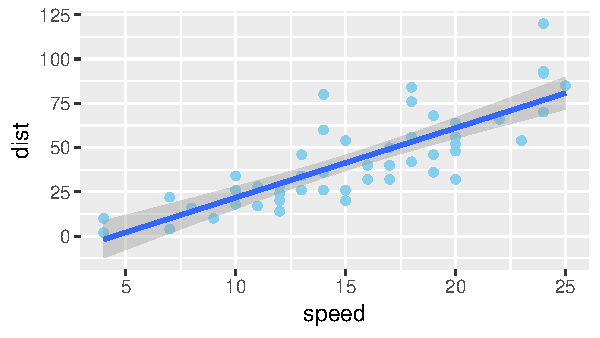
\includegraphics[width=\textwidth]{plots/myplot1.pdf}
        \caption{A plot with blue dots.}
        \label{fig:PlotBlue}
    \end{subfigure}
    \hfill
  \begin{subfigure}[b]{0.45\textwidth}
        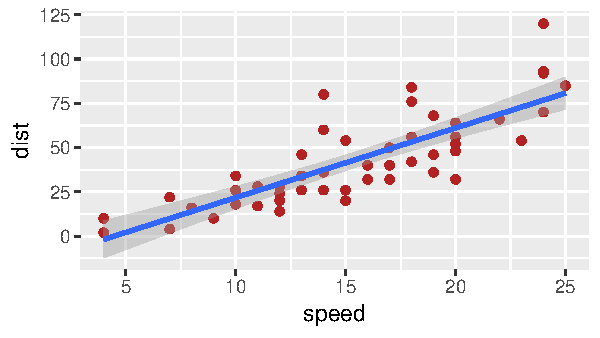
\includegraphics[width=\textwidth]{plots/myplot2.pdf}
        \caption{A plot with red dots.}
        \label{fig:PlotRed}
    \end{subfigure}
  \caption{A figure with subfigures.}
  \label{fig:Plot}
\end{figure}

\section*{Numerical results}

\subsection*{Number formatting}

The \texttt{siunitx} package offers a lot of room for typesetting numbers and units. Here, two
convenience functions are defined on top of the functionality provided by this package:
\verb|\rlnum{}{}| and \verb|\rlnumsci{}{}|. To get a rounded number, we can use
\verb|\rlnum{1312.31003}{2}| which produces \rlnum{1312.31003}{2}. The second argument gives
the number of rounding integers after the comma, so that \verb|\rlnum{1312.31003}{3}| yields
\rlnum{1312.31003}{3}. We get scientific notation with \verb|\rlnumsci{1312.31003}{3}| to
obtain \rlnumsci{1312.31003}{3}.

\subsection*{Single numbers from CSV files}

Results from computations in R are stored in CSV files. The \texttt{csvsimple} package allows
to manipulate data from CSV files in many ways. Here, three simple wrapper functions are defined on
top of this package. Each one of the functions:
\begin{verbatim}
 \rlgetvalue{FILENAME.CSV}{COLNAME-KEYS}{KEY}{COLNAME-VALUE}
 \rlgetnum{FILENAME.CSV}{COLNAME-KEYS}{KEY}{COLNAME-VALUE}{PRECISION}
 \rlgetnumsci{FILENAME.CSV}{COLNAME-KEYS}{KEY}{COLNAME-VALUE}{PRECISION}
\end{verbatim}
loads the file \texttt{FILENAME.CSV}, finds all rows in which the entry for the column
\texttt{COLNAME-KEYS} matches the string in \texttt{KEY} and returns the value of that row from
column \texttt{COLNAME-VALUE}. The difference between these three functions is:
\begin{itemize}
\item \texttt{rlgetvalue} returns what is in the CSV file exactly as it is, be it string or
  number; all formatting needs to be done in R;
\item \texttt{rlgetnum} and \texttt{rlgetnumsci} expect a numerical entry and pipe it into
  \verb|\rlnum{}{}| and \verb|\rlnumsci{}{}| respectively; they therefore take an additional
  \texttt{PRECISION} argument. 
\end{itemize}

For example, the data in file \texttt{R\_data\_4\_TeX/mystats1.csv} looks like this:
\begin{verbatim}
  variable,mean,sd              
  dist,42.98,25.769377492025892 
  speed,15.4,5.2876444352347844 
\end{verbatim}
A call of \verb|\rlgetnum{mystats1.csv}{variable}{dist}{sd}{2}| gives
\rlgetnum{mystats1.csv}{variable}{dist}{sd}{2}.\footnote{Notice that the first argument of all
  of these functions should specify the full, relative path to the relevant CSV file. However,
  it is convenient to define specify the path to a folder where all relevant CSV files are
  found globally using a \LaTeX\ command, as done in this example (see source code and comments
  therein), so that we do not need to specify the folder name
  with each retrieval command.} \\
A call of \verb|\rlgetvalue{R_data_4_TeX/mystats1.csv}{variable}{dist}{sd}| gives
\rlgetvalue{mystats1.csv}{variable}{dist}{sd}.

If there are several rows in the CSV file that match the filter, these convenience functions
will output a list of all values retrieved. So, if the data rather looked like in file
\texttt{mystats2.csv}:
\begin{verbatim}
  variable,stat,value        
  dist,mean,42.98            
  speed,mean,15.4            
  dist,sd,25.769377492025892 
  speed,sd,5.2876444352347844
\end{verbatim}
we get \rlgetnum{mystats2.csv}{variable}{dist}{sd}{2} from \verb|\rlgetnum{mystats2.csv}{variable}{dist}{sd}{2}|. 

\subsection*{Tables of numerical results}

The \texttt{csvsimple} package allows typesetting tables from CSV files, but the
\texttt{pgfplotstable} package allows for even more flexibility. As an example, we plot the
outcome of a regression analysis stored in file \texttt{mytable.csv}, which is reproduced here:
\begin{verbatim}
  Rowname,Estimate,Std. Error,t value,Pr(>|t|)                                         
  (Intercept),-17.579094890510877,6.758440169379233,-2.601058003022246,0.01231881615380909
  speed,3.9324087591240846,0.41551277665712216,9.463989990298366,1.4898364962950983e-12
\end{verbatim}
A nice format for this data is in Table~\ref{tab:MyTable}, which is produced by the code in Figure~\ref{fig:Code}.

\begin{center}
  \begin{table}[h]
    \centering

    \pgfplotstabletypeset[sci zerofill,
    col sep = comma,
    every head row/.style={before row = \toprule, after row = \midrule},
    every last row/.style={after row = \bottomrule},
    columns/Rowname/.style={string type, column name={}, column type = l},
    columns/Estimate/.style={column name={Estimate}, dec sep align},
    columns/Std. Error/.style={column name={SDE}, sci sep align, sci},
    columns/t value/.style={column name={$t$-value}, dec sep align},
    columns/Pr(>|t|)/.style={column name={$p$-value}, dec sep align }]
    {R_data_4_TeX/mytable.csv}

    \caption{A table generated from a CSV-file with the code in Figure~\ref{fig:Code}.}
    \label{tab:MyTable}
  \end{table}
\end{center}

\begin{figure}[t]
  \centering
  \begin{verbatim}
   \pgfplotstabletypeset[sci zerofill,
   col sep = comma,
   every head row/.style={before row = \toprule, after row = \midrule},
   every last row/.style={after row = \bottomrule},
   columns/Rowname/.style={string type, column name={}, column type = l},
   columns/Estimate/.style={column name={Estimate}, dec sep align},
   columns/Std. Error/.style={column name={SDE}, sci sep align, sci},
   columns/t value/.style={column name={$t$-value}, dec sep align},
   columns/Pr(>|t|)/.style={column name={$p$-value}, dec sep align }]
   {R_data_4_TeX/mytable.csv}
  \end{verbatim}
  \caption{Code that produced Table~\ref{tab:MyTable}.}
  \label{fig:Code}
\end{figure}

\subsection*{Individual unrelated variables}

On top of information about numerical variables that are related in an obvious way (and are
therefore gathered logically in a data frame), we may want to have an assorted list of
independent variables, like the number of participants, the average error rate, the mean rating
of a post-survey question etc. In the script \verb|R_code.r| we gather these in a list, which
is handy because these variables might occur at several places in a script. We finally save
this list as a CSV file in long format (each column is a variable, with one row containing the
variables' values). It is handy to have the same format and name for this CSV file across
different projects, like here: \verb|myvars.csv|.

We can then insert the value of a single variable like \texttt{maxSpeed} with command
\verb|\rlgetvariable{maxSpeed}|, which produces: \rlgetvariable{maxSpeed}. This also works for strings: the
result of \verb|\rlgetvariable{someString}| is \rlgetvariable{someString} 

\section*{ToDos}

\begin{itemize}
\item scientific notation not uniform in Table~\ref{tab:MyTable}
\item OSF show up with \verb|rlgetvariable| but not with the other techniques
\end{itemize}

\printbibliography[heading=bibintoc]

\end{document}
